
\documentclass{abgabe}

\newcommand{\Schlaf}{\text{Schlaf}}
\newcommand{\Note}{\text{Note}}

\begin{document}

\begin{questions}
    \question
    Die Schülerinnen und Schüler wurden vor der Klausur anonym befragt, wie viele Stunden Schlaf sie vor der Klausur gehabt haben:
    \begin{center}
        \begin{tabular}{|c||C|C|C|C|C|C|C|C|C|C|}
            \hline
            Note   & 2 & 4 & 3 & 5 & 6 & 6 & 1 & 2 & 5 & 4 \\
            \hline
            Schlaf & 9 & 5 & 6 & 5 & 1 & 2 & 9 & 8 & 4 & 7 \\
            \hline
        \end{tabular}
    \end{center}

    \begin{parts}
        \part
        Berechnen Sie aus den Daten
        \begin{subparts}
            \subpart
            die empirische Kovarianz
            \begin{solution}
                $N$ und $S$ seien wie offensichtlich definiert. TO DO: Umbenennen in X und Y

                Es gilt:
                \[
                    \Cov(X, Y) = s_{XY} = \frac{1}{n-1} \cdot \sum_{i=1}^{n} (x_i - \conj{x})(y_i - \conj{y}) = \frac{1}{n-1} \left( \sum_{i=1}^{n} x_iy_i - n \cdot \conj{x} \cdot \conj{y} \right)
                \]

                Wir berechnen zuerst die arithmetischen Mittel von $X$ und $Y$ wie folgt:
                \[
                    \conj{x} = \frac{1}{n} \sum_{i=1}^n x_i = \frac{1}{10} \cdot (2 + 4 + 3 + 5 + 6 + 6 + 1 + 2 + 5 + 4) = \frac{19}{5} = 3.8
                \]
                \[
                    \conj{y} = \frac{1}{n} \sum_{i=1}^n y_i = \frac{1}{10} \cdot (9 + 5 + 6 + 5 + 1 + 2 + 9 + 8 + 4 + 7) = \frac{28}{5} = 5.6
                \]

                Damit gilt:
                \begin{alignat*}{1}
                    \Cov(X, Y) = s_{xy} & = \frac{1}{n-1} \cdot \sum_{i=1}^{n} (x_i - \conj{x})(y_i - \conj{y})                         \\
                                        & = \frac{1}{n-1} \left( \sum_{i=1}^{n} x_iy_i - n \cdot \conj{x} \cdot \conj{y} \right)        \\
                                        & = \frac{1}{9} \left( \sum_{i=1}^{n} x_iy_i - 10 \cdot \frac{19}{5} \cdot \frac{28}{5} \right) \\
                                        & = \frac{1}{9} \left( \sum_{i=1}^{n} x_iy_i - \frac{1064}{5} \right)                           \\
                                        & = \frac{1}{9} \sum_{i=1}^{n} x_iy_i - \frac{1064}{45}                                         \\
                                        & = \frac{1}{9} \cdot 172 - \frac{1064}{45}                                                     \\
                                        & = -\frac{68}{15} \approx -4.53
                \end{alignat*}
                \qed
            \end{solution}

            \newpage
            \subpart
            den empirischen Korrelationskoeffizient
            \begin{solution}
                Es gilt:
                \[
                    r_{xy} = \frac{s_{xy}}{s_x \cdot s_y} = \frac{\sum_{i=1}^{n} (x_i - \conj{x})(y_i - \conj{y})}{\sqrt{\sum_{i=1}^{n} (x_i - \conj{x})^2 \cdot \sum_{i=1}^{n} (y_i - \conj{y})^2 }}
                \]
                Wir berechnen zuerst die empirischen Standardabweichungen $s_x$ und $s_y$ von $X$ und $Y$ wie folgt:
                \[
                    s_x^2 = \frac{1}{n-1} \sum_{i=1}^{n} (x_i - \conj{x})^2 = \frac{1}{9} \sum_{i=1}^{n} \left(x_i - \frac{19}{5} \right)^2 = \frac{46}{15} \implies s_x = \sqrt{\frac{46}{15}} = \frac{\sqrt{690}}{15}
                \]
                \[
                    s_y^2 = \frac{1}{n-1} \sum_{i=1}^{n} (y_i - \conj{y})^2 = \frac{1}{9} \sum_{i=1}^{n} \left(y_i - \frac{28}{5} \right)^2 = \frac{38}{5} \implies s_y = \sqrt{\frac{38}{5}} = \frac{\sqrt{190}}{5}
                \]

                Damit gilt dann:
                \[
                    r_{xy} = \frac{s_{xy}}{s_x \cdot s_y} = \frac{-\nicefrac{68}{15}}{\nicefrac{\sqrt{690}}{15} \cdot \nicefrac{\sqrt{190}}{5}} = - \frac{34\sqrt{1311}}{1311} \approx -0.93903
                \]
                \qed
            \end{solution}

            \subpart
            die lineare Regression
            \begin{solution}
                Die Regressionsgerade ist gegeben mit
                \[
                    \hat{y}_i = \hat{a} + \hat{b}x
                \]

                Es gilt:
                \[
                    \hat{b} = \frac{s_{xy}}{s_x^2} = \frac{-\nicefrac{68}{15}}{\nicefrac{46}{15}} = - \frac{34}{23} \approx -1.478
                \]
                \[
                    \hat{a} = \conj{y} - \hat{b} \cdot \conj{x} = \frac{28}{5} + \frac{34}{23} \cdot \frac{19}{5} = \frac{258}{23} \approx 11.217
                \]
                \qed
            \end{solution}
        \end{subparts}

        \newpage
        \part
        Erstellen Sie ein Streudiagramm und zeichnen Sie die Regressionsgerade ein.
        \begin{solution}

            \begin{center}
                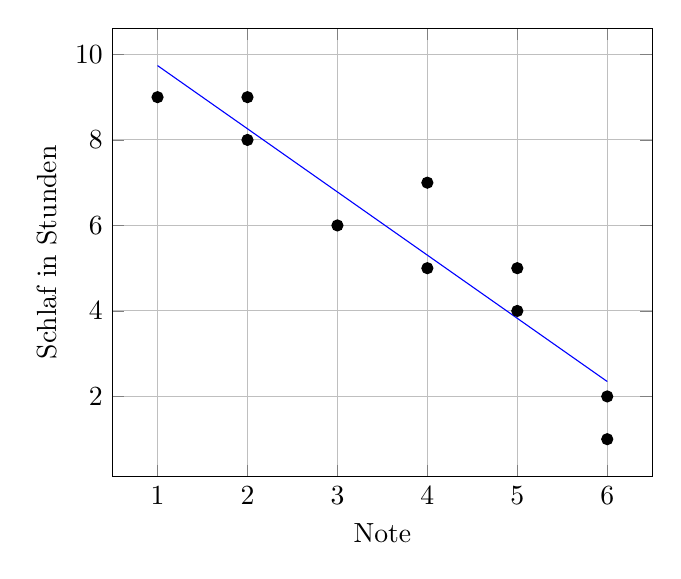
\begin{tikzpicture}
                    \begin{axis}[%
                            grid=both,
                            xlabel={Note},
                            ylabel={Schlaf in Stunden},
                            scatter/classes={%
                                    a={mark=o,draw=black}}]
                        \addplot[scatter,only marks,%
                            scatter src=explicit symbolic]%
                        table {
                                x y
                                2 9
                                4 5
                                3 6
                                5 5
                                6 1
                                6 2
                                1 9
                                2 8
                                5 4
                                4 7
                            };
                        \addplot[domain=1:6, color=blue]{11.217 -1.478 * x};
                    \end{axis}
                \end{tikzpicture}
            \end{center}
            \qed
        \end{solution}
    \end{parts}
\end{questions}
\end{document}